\documentclass[3p,sort&compress,11pt,fleqn,review]{elsarticle}
\bibliographystyle{elsarticle-num-names}
\usepackage{amsmath,amsfonts,amssymb,siunitx,float,subcaption,setspace,booktabs,bm,mathtools,url,algorithm,algpseudocode,lineno,lmodern}
\usepackage[fixed]{fontawesome5}
%\usepackage{easyReview}
\journal{}
\newcommand{\balpha}{\mb{\alpha}}
\newcommand{\bbeta}{\mb{\beta}}
\newcommand{\bc}{\mb{c}}
\newcommand{\bd}{\mb{d}}
\newcommand{\be}{\mb{e}}
\newcommand{\beeta}{\mb{\eta}}
\newcommand{\bgamma}{\mb{\gamma}}
\newcommand{\bn}{\mb{n}}
\newcommand{\bq}{\mb{q}}
\newcommand{\bs}{\mb{s}}
\newcommand{\bsigma}{\mb{\sigma}}
\newcommand{\bv}{\mb{v}}
\newcommand{\bvarepsilon}{\mb{\varepsilon}}
\newcommand{\bzeta}{\mb{\zeta}}
\newcommand*{\algoref}[1]{Algorithm~\ref{#1}}
\newcommand*{\ddfrac}[2]{\dfrac{\md{#1}}{\md{#2}}}
\newcommand*{\dev}[1]{\text{dev}\left(#1\right)}
\newcommand*{\diag}[1]{\text{diag}\left(#1\right)}
\newcommand*{\eqsref}[1]{Eq.~(\ref{#1})}
\newcommand*{\figref}[1]{Fig.~\ref{#1}}
\newcommand*{\mb}[1]{\bm{#1}}
\newcommand*{\md}[1]{\mathrm{d}#1}
\newcommand*{\mdd}[1]{\mathrm{d}^2#1}
\newcommand*{\mT}{\mathrm{T}}
\newcommand*{\pdfrac}[2]{\dfrac{\partial{#1}}{\partial{#2}}}
\newcommand*{\secref}[1]{\S~\ref{#1}}
\newcommand*{\sign}[1]{\text{sign}\left(#1\right)}
\newcommand*{\tabref}[1]{Table~\ref{#1}}
\DeclarePairedDelimiter\abs{\lvert}{\rvert}
\DeclarePairedDelimiter\norm{\lVert}{\rVert}
\makeatletter
\let\oldabs\abs\def\abs{\@ifstar{\oldabs}{\oldabs*}}
\let\oldnorm\norm\def\norm{\@ifstar{\oldnorm}{\oldnorm*}}
\newenvironment{breakablealgorithm}{\begin{center}\refstepcounter{algorithm}\hrule height.8pt depth0pt \kern2pt
\renewcommand{\caption}[2][\relax]{
{\raggedright\textbf{\ALG@name~\thealgorithm} ##2\par}
\ifx\relax##1\relax
\addcontentsline{loa}{algorithm}{\protect\numberline{\thealgorithm}##2}
\else
\addcontentsline{loa}{algorithm}{\protect\numberline{\thealgorithm}##1}
\fi
\kern2pt\hrule\kern2pt}}{\kern2pt\hrule\relax\end{center}}
\makeatother
\begin{document}
\linenumbers
\begin{abstract}
    \begin{linenumbers}
        In this work, we revisit the subloading surface model, as well as its extended version.
        By investigating its original formulation, we provide an alternative interpretation.
        With which, it is shown that the corresponding evolution rules of historic variables can be greatly simplified.
        The proposed evolution rules are analytically more concise and possess straightforward implications that can be easily illustrated while remain mathematically equivalent to the original ones.
        Based on the new proposal, an implicit numerical algorithm is presented.
        Compared to the previous implementation, the new algorithm is more efficient and robust.
        Additional insights regarding the unconventional (un)loading criterion and the specific form of some functions are also discussed.
    \end{linenumbers}
\end{abstract}
\begin{keyword}
    constitutive modelling\sep
    plasticity\sep
    subloading surface model\sep
    ratcheting\sep
    cyclic response
\end{keyword}
\begin{frontmatter}
    \title{On the Subloading Surface Model for Metals: Some Insights and an Efficient Numerical Implementation}
    \author[add1]{Theodore~L.~Chang\corref{tlc}}\ead{tlcfem@gmail.com}
    \cortext[tlc]{corresponding author}
    \address[add1]{IRIS Adlershof, Humboldt-Universität zu Berlin, Berlin, Germany, 12489.}
\end{frontmatter}
\section{Introduction}
The conventional plasticity theory adopts the concept of yield/loading surface \citep[see, e.g.,][]{Lemaitre1990,Simo1998} to describe the onset of plastic deformation.
The surface encloses a region where the material is elastic, and once the stress state reaches the surface, plastic deformation occurs.
Because of this clear distinction between elastic and plastic states, the corresponding stiffness is often discontinuous when transiting from elastic to plastic states.
Although such a discontinuity is not physically sound, this is often not a concern for most models as the capability of capturing more accurate cyclic responses (and/or other objectives) is often more important, especially for metals.
To this end, models employ advanced/modified kinematic hardening rules enriched with various types of rate control and hardening activation/deactivation, such as Ohno's modifications \citep[see, e.g.,][]{Ohno1982,Ohno1993,Ohno2021} and Yoshida's modification \citep{Yoshida2002}, based on the famous Armstrong--Frederick rule \citep{Frederick2007} and its multiplicative version, see a comprehensive review by \citet{Chaboche2008}, have been proposed.
However, models of this kind often present decent cyclic responses under two--sided cyclic loading but are \emph{`incapable of describing the \textnormal{(general, including one--sided and small cycles)} cyclic loading behaviour'} \citep[][pg. 282]{Hashiguchi2023} due to the existence of the elastic region, regardless of large or small \citep{Dafalias1977}.

On the contrary, the subloading surface model offers a quite unique approach that is different from the conventional framework.
The initial proposal of the subloading surface model can be dated back to the work by \citet{Hashiguchi1980}.
The model is later extended \citep{Hashiguchi1989} to include an elastic core, which enables the model to describe more versatile cyclic responses.
Over the decades of development, it has been widely adopted in various applications, to name a few recent endeavours, see the work by \citet{Maranha2016,Xiong2018,Anjiki2021,Yamakawa2021,Yamakawa2022,Lu2023}.
The comprehensive review of the subloading surface model and its extended version can be found in the recent review papers by \citet{Hashiguchi2023a} and \citet{Hashiguchi2024}.
Meanwhile, the classification and overview of plasticity models is summarised and well documented in the monograph by \citet[see][\S~10.2]{Hashiguchi2023}.
Interested readers are referred to these references for more detailed information.

The (extended) subloading surface model possesses many advantages over conventional plasticity models.
The most notable one is that it provides a smooth transition between elastic and plastic states, implying the tangent stiffness is continuous under all loading conditions.
Such a continuity is more realistic and tends to be beneficial not only for static analyses, but also for other applications such as damping formulation, for example, a stiffness proportional damping based on the tangent stiffness matrix would now result in a continuous damping matrix, thus, a continuous damping force.
Furthermore, due to the introduction of the elastic core in the extended version, it is much more capable of describing ratcheting behaviour under cyclic loading, which cannot be well captured by conventional models that incorporate a pure elastic region.

The choice of internal history variables in the existing formulation bears a clear and straightforward physical implication.
However, their evolution rules \citep[see, e.g.,][]{Hashiguchi2024} appear to be somewhat cumbersome and not very intuitive.
Due to the same reason, the corresponding numerical implementation \citep[see, e.g.,][]{Fincato2017,Anjiki2019,Anjiki2021} involves a local system possessing a significant size (around \num{20} for 3D models).
Thus, it appears to be less efficient and robust.
In this work, we focus on the following three tasks:
\begin{enumerate}
    \item revise the definition(s) and the corresponding evolution rule(s) of some key internal history variables to make them concise and intuitive both analytically and numerically;
    \item propose a concise and universal loading/unloading criterion that is cheap to evaluate and can be easily implemented;
    \item improve numerical stability by discussing and choosing more numerical friendly functions for the evolution rules.
\end{enumerate}
As a showcase, a reference algorithm is also presented which adopts the von Mises framework that is suitable for metals.

The paper is organized as follows.
The original formulation of the (extended) subloading surface model is briefly reviewed in \secref{sec:subloading}.
Based on which, a revised formulation with improved evolution rules and loading/unloading criterion is proposed in \secref{sec:revised}.
A reference implementation for von Mises materials is presented thereafter.
Numerical analyses cover the comparison between the conventional and the proposed (un)loading criterion and the accuracy analysis of the proposed algorithm.
\section{The Extended Subloading Surface Model}\label{sec:subloading}
In this section, the framework of the (extended) subloading surface model is briefly reviewed and summarised.
\subsection{The Subloading Surface}
Conventional plasticity models often adopt the concept of a yield surface, denoted by $f\left(\bsigma,\cdots\right)$, which defines the frontier/boundary of plasticity.
For example,
\begin{gather}
    f=\norm{\beeta}-F,
\end{gather}
in which $\beeta=\beeta\left(\bsigma,\cdots\right)$ is known as the shifted stress that shall be a function of the stress tensor $\bsigma$ and other internal variables, $F=F\left(q\right)$ characterises the size of this surface and could evolve with the development of plasticity driven by some internal variable $q$.
Within the yield surface $f$, the material is elastic, while plasticity would develop once the stress state reaches and exceeds $f$, in which case, the surface itself would also expand to enclose the current stress state accordingly.
Thus, any admissible state shall satisfy the inequality $f\leqslant0$.

The original proposal of the subloading surface model introduces a new internal variable, named as the normal yield ratio, denoted by $z$ in this work, which effectively scales the yield surface $f$ down by a factor $z$, the new surface is call the subloading surface $f_s$ and it is concentric with the yield surface $f$.
\begin{gather}
    f_s=\norm{\beeta}-zF.
\end{gather}
The normal yield ratio $0\leqslant{}z\leqslant{}1$ shall be updated in a manner such that $f_s=0$ is enforced not only for plastic loading but also for elastic unloading.
With such a construct, any given stress state would always lie on the subloading surface, meaning that $f_s=0$ is always satisfied.

The main shortcoming of the original subloading surface model is that it exhibits excessive strain accumulation under cyclic loading.
To address this issue, an additional internal field, denoted by $\bc$, is adopted to define the elastic core surface in the extended subloading surface model, which is concentric with the yield surface (centred at the back stress $\bbeta$).
The subloading surface is then pulled from the original centre $\bbeta$ towards $\bc$ by a certain amount governed by the normal yield ratio $z$.
\begin{figure}[htb]
    \centering
    \includegraphics[page=1]{PICCOLLECTION}
    \caption{graphical representation of the surfaces used in the subloading surface model}\label{fig:surfaces}
\end{figure}
A graphical illustration is shown in \figref{fig:surfaces}.
By definition, $\bc$ denotes the homothetic centre between $f$ and $f_s$.
Then, according to similarity, the new centre of the subloading surface is $\bbeta+\left(1-z\right)\left(\bc-\bbeta\right)$, that is $z\bbeta+\left(1-z\right)\bc$.
\subsection{Original Evolution Rules}
The evolution rule for the elastic core has undergone several iterations, see, for example, the initial version \citep{Hashiguchi1989}, one of the variations \citep{Hashiguchi2015}, the most recent version \citep{Anjiki2019}.
The original formulation further imposes the requirement that the size of the elastic core shall be limited to a certain fraction of that of the yield surface.
This is achieved by the following evolution rule for $\bc$ \citep{Anjiki2019,Hashiguchi2023},
\begin{gather}\label{eq:original_core}
    \dot{\bc}=c_e\gamma\left(z_eF\bn-\left(\bc-\bbeta\right)\right)+\dot{\bbeta}+\dfrac{\dot{F}}{F}\left(\bc-\bbeta\right).
\end{gather}
In which, $0\leqslant{}c_e$ is a constant that controls the evolution rate, $0\leqslant{}z_e\leqslant1$ is a constant that controls the limit size of the elastic core, $\gamma$ is the plastic multiplier and $\bn=\pdfrac{f_s}{\bsigma}/\norm{\pdfrac{f_s}{\bsigma}}$ is unit gradient of the subloading surface.

The evolution rule for the normal yield ratio $z$ is given by
\begin{gather}\label{eq:original_z}
    \dot{z}=U\dot{q},
\end{gather}
where $U=U\left(z\right)$ is a function that shall satisfy certain conditions, and $q$ is the accumulated plastic strain.

Both of the above evolution rules will be discussed and refined in the following sections.
Here, we only present them in their original forms for completeness.
\section{A Revised Formulation}\label{sec:revised}
\subsection{Preliminary Remarks}
In the scalar form, the Armstrong--Frederick evolution rule \citep{Frederick2007} is equivalent to the following ordinary differential equation (ODE),
\begin{equation}\label{eq:af_ode}
    y'=b\left(a-y\right),
\end{equation}
it can be explicitly integrated to give the solution for the initial condition $y(0)=0$,
\begin{equation}
    y(x)=a\left(1-\exp\left(-bx\right)\right),
\end{equation}
which defines a curve that asymptotically approaches the constant bound $a$.

To employ a non-constant bound, it is possible to simply replace the constant $a$ by a function $a(x)$ in the ODE \eqsref{eq:af_ode} such that $y'=b\left(a\left(x\right)-y\right)$.
However, as noted in the literature, the corresponding solution is not strictly bounded by $a(x)$.
\figref{fig:examples} presents both hardening and softening examples to illustrate this point.
\begin{figure}[htb]
    \centering
    \begin{subfigure}{.48\textwidth}
    \centering
    \includegraphics[page=2]{PICCOLLECTION}
    \caption{softening}
    \end{subfigure}\hfill
    \begin{subfigure}{.48\textwidth}
    \centering
    \includegraphics[page=3]{PICCOLLECTION}
    \caption{hardening}
    \end{subfigure}
    \caption{asymptotic behaviour with hardening and softening bounds}\label{fig:examples}
\end{figure}
As can be seen from the figure, the solution may overshoot for softening bounds.
Furthermore, in both cases, the solution $y$ does \textbf{not} asymptotically approach the bound $a(x)$.
That is, the following condition does not hold for arbitrarily small $\epsilon$,
\begin{gather}
    \lim\limits_{x\to\infty}\abs{y-a(x)}<\epsilon.
\end{gather}
It is worth noting that the following form
\begin{gather}
    y'=b\left(1-\dfrac{1}{a\left(x\right)}y\right)=\dfrac{b}{a\left(x\right)}\left(a\left(x\right)-y\right)
\end{gather}
has a similar solution to that of $y'=b\left(a\left(x\right)-y\right)$.
The $y'$ is governed by the difference $a\left(x\right)-y$, while the approaching rate changes from $b$ to $b/a\left(x\right)$.
They are equivalent in terms of the asymptotic behaviour and share the same shortcoming.
This form has been used in defining the evolution rule for the back stress in the subloading surface model \citep[see, e.g.,][]{Anjiki2019,Hashiguchi2023,Hashiguchi2024}.

To ensure that the solution is bounded by $a(x)$, let's consider the following function,
\begin{gather}\label{eq:strict_bound_core}
    y=a(x)\left(1-\exp\left(-bx\right)\right),
\end{gather}
since $1-\exp\left(-bx\right)<1$, it is guaranteed that $y<a(x)$.
On the other hand, the corresponding ODE can be derived as follows,
\begin{gather}\label{eq:strict_bound}
    y'=ab\exp\left(-bx\right)+a'\left(1-\exp\left(-bx\right)\right)=b\left(a-y\right)+\dfrac{a'}{a}y.
\end{gather}
After careful comparison, one could observe that \eqsref{eq:strict_bound} is in fact the scalar unidirectional version of the evolution rule presented in \eqsref{eq:original_core}.
They bear the same format.
Thus, one can conclude that \eqsref{eq:strict_bound_core} is mathematically equivalent to \eqsref{eq:strict_bound} as it is the solution to the latter with the initial condition $y(0)=0$, however, the latter is much more cumbersome.
\subsubsection{Revised Evolution Rule (Elastic Core)}
The evolution rule for $\bc$ shown in \eqsref{eq:original_core} is derived at the limit state where the subloading surface coincides with the limit surface --- which would not occur due to its asymptotic nature.
It possesses a cumbersome form that involves both $F$ and its derivative.
As a result, it is not straightforward to implement numerically.
Instead, based on the above observations, one can apply the following decomposition,
\begin{gather}\label{eq:decomposition_core}
    \boxed{\bc-\bbeta=F\bd\qquad\rightarrow\qquad\bc=\bbeta+F\bd,}
\end{gather}
with $F\bd$ characterises the size of the elastic core surface, then the evolution of $\bc$, which characterises a point on the elastic core surface, can be equivalently described by the evolution of $\bd$, which could take a very simple form as the contribution of $F$ is separated,
\begin{gather}\label{eq:revised_core}
    \boxed{\dot{\bd}=c_e\left(z_e\bn-\bd\right)\gamma.}
\end{gather}
Since the magnitude of $\bd$ defined in this manner is bounded by the constant $z_e$, it is then guaranteed that $\norm{\bc-\bbeta}=F\norm{\bd}<z_eF$.
Based on the above discussion, it can be asserted that \eqsref{eq:revised_core} is mathematically equivalent to \eqsref{eq:original_core}.
However, such a decomposition separates the directional vector from the scalar magnitude, which allows much simpler evolution rules for both parts, although the vector here is not a unit vector thus does not possess a fixed unit length.
\eqsref{eq:decomposition_core} may be called the `\textit{pseudo-polar coordinate}' representation while $\bd$ may be called the `\textit{similarity vector}' as it points to the similarity centre $\bc$.
\subsubsection{Revised Evolution Rule (Back Stress)}
Now since \eqsref{eq:decomposition_core} is adopted, a similar strategy can also be applied to $\bbeta$ to allow its bound to evolve with the development of plasticity, that is,
\begin{gather}\label{eq:decomposition_back}
    \boxed{\bbeta=H\balpha,}
\end{gather}
with $H=H\left(q\right)$ being the bound and $\balpha$ being the normalised back stress (normalised by $H$) which could have the following evolution rule.
\begin{gather}\label{eq:revised_back}
    \boxed{\dot{\balpha}=b\left(\bn-\balpha\right)\gamma,}
\end{gather}
where $b$ is a constant that controls the evolution rate.
Similar to $\norm{\bc-\bbeta}$, here it is guaranteed that $\norm{\bbeta}=H\norm{\balpha}<H$.

It is possible to associate $H$ with $F$ such that $H$ is set to a fraction of $F$.
Here, to allow more flexibility, $H$ is defined as an independent quantity.
Nevertheless, if one wishes, it is possible to associate $H$ with $F$ as done in other work \citep[e.g.,][]{Anjiki2019}.
However, one shall note that the specific form $\bbeta=b\left(\bn-\dfrac{\bbeta}{H}\right)\gamma$ shall not be used for the same reason as discussed previously, see \figref{fig:examples}.
\subsubsection{Shifted Stress}
Since now the new centre of the subloading surface is shifted to $\bbeta+\left(1-z\right)\left(\bc-\bbeta\right)$, the original formulation uses the following expression to compute the shifted stress $\beeta$,
\begin{gather}
    \beeta=\bs-\left(\bbeta+\left(1-z\right)\left(\bc-\bbeta\right)\right),
\end{gather}
where $\bs=\bs\left(\bsigma\right)$ is some function of the stress tensor.
Account for the proposed decompositions \eqsref{eq:decomposition_core} and \eqsref{eq:decomposition_back}, the above expression can be rewritten as
\begin{gather}
    \boxed{\beeta=\bs-H\balpha+\left(z-1\right)F\bd,}
\end{gather}
\figref{fig:revised_surfaces} presents a graphical representation of the quantities used in this revised formulation.
\begin{figure}[htb]
    \centering
    \includegraphics[page=4]{PICCOLLECTION}
    \caption{graphical representation of the surfaces using proposed definitions}\label{fig:revised_surfaces}
\end{figure}
It could also be noted that, since $\norm{\bd}<1$, then $\norm{zF\bd}<zF$, the homothetic centre is always inside the subloading surface $f_s$, which itself is inside the yield surface $f$.
\subsubsection{Loading/Unloading Criterion}\label{sec:correct_loading_criterion}
The conventional Kuhn--Tucker condition cannot be applied in the subloading surface model since, even for elastic unloading, the history variable $z$ shall be updated for every load increment/step.
For arbitrary loading directions and magnitudes, there exists possibilities that the normal yield ratio $z$ may decrease first --- the subloading surface shrinks, then increase --- the subloading surface expands.
When it expands, the plasticity can only be correctly computed with the correct initial value of $z$.
An inward load increment resulting in $f_s^\text{trial}<0$ does not necessarily imply that it is a pure elastic unloading step.
A graphical representation is shown in \figref{fig:loading_criterion}.
\begin{figure}[htb]
    \centering
    \includegraphics[page=5]{PICCOLLECTION}
    \caption{arbitrary loading direction with frozen plasticity}\label{fig:loading_criterion}
\end{figure}

In the trial state, by freezing plasticity, viz., $H$, $F$, $\balpha$ and $\bd$ are all kept constant, it can be concluded that the centre of the subloading surface must lie on the line defined by centre of the yield surface $\bbeta$ and the similarity centre $\bc=\bbeta+F\bd$.
Then, for a given load increment $\Delta\bs=\bs_{n+1}-\bs_n$, assuming proportional loading, there exists a scalar $r$ such that the corresponding stress state $\bs_n+r\Delta\bs$ would minimise $z$, we denote this $z$ as $z^\text{trial}$ since it is computed in the trial state.
In mathematical terms, it can be expressed as
\begin{gather}
    \boxed{\min\limits_{r\in\mathbb{R}}z^\text{trial}\qquad\text{s.t.}\qquad{}f_s^\text{trial}\left(z^\text{trial},r\right)=0,}
\end{gather}
where $z^\text{trial}$ shall be computed by enforcing the corresponding $f_s^\text{trial}=0$.
% \begin{gather}\label{eq:trial_criterion}
%     \begin{split}
%         f_s^\text{trial} & =\norm{\beeta^\text{trial}}-z^\text{trial}F_n                                                 \\
%                          & =\norm{\bs_n+r\Delta\bs-H_n\balpha_n+\left(z^\text{trial}-1\right)F_n\bd_n}-z^\text{trial}F_n \\
%                          & =\norm{\bar{\beeta}+z^\text{trial}F_n\bd_n}-z^\text{trial}F_n                                 \\
%                          & =0,
%     \end{split}
% \end{gather}
% in which $\bar{\beeta}=\bar{\beeta}\left(r\right)=\bs_n-H_n\balpha_n-F_n\bd_n+r\Delta\bs$.
% The subscript $\left(\cdot\right)_n$ denotes the converged state at the beginning of the current loading step.
Since no extra constraints are imposed on $r$ for the moment, a solution is guaranteed to exist.
However, there are three distinctive cases.
\begin{enumerate}
    \item If $0<r<1$, the given load increment $\Delta\bs$ contains both elastic unloading and plastic loading.
          Since the elastic unloading portion ($0\to{}r$) reduces $z$ to a value smaller than the converged $z_n$, the plastic loading portion ($r\to{}1$) shall use this minimum $z$ (smaller than $z_n$, not necessarily zero in 3D models), instead of $z_n$, as the starting value to correctly compute plasticity development.
    \item If $r\geqslant1$, the given load increment $\Delta\bs$ involves only elastic unloading.
    \item If $r\geqslant0$, it is a pure loading case. Nothing additional needs to be done. $z_n$ is the correct starting value for return mapping.
\end{enumerate}
Thus, for any given load increment, one could 1) find the corresponding scalar $r$ that minimises $z^\text{trial}$, 2) use the above criteria to determine whether plasticity occurs, if so, also correct the starting value of $z$ if necessary.
We defer the presentation of explicit expressions for the above procedure after introducing the von Mises framework.
\subsection{A von Mises Material Model}
In the following, we present discrete expressions within the von Mises framework.
\subsubsection{Subloading Surface}
For the von Mises criterion, $\bs$ shall take the deviatoric part of the stress tensor $\bs=\dev{\bsigma}$, then
\begin{gather}
    \beeta=\dev{\bsigma}-H\balpha+\left(z-1\right)F\bd.
\end{gather}
The subloading surface shall be expressed as follows by replacing $F$ with $\sqrt{\dfrac{2}{3}}\sigma^y$.
\begin{gather}\label{eq:mises_subloading_surface}
    f_s=\norm{\beeta}-z\sqrt{\dfrac{2}{3}}\sigma^y.
\end{gather}
\subsubsection{Flow Rule}
Assuming associative plasticity, the flow rule is given by
\begin{gather}\label{eq:subloading_flow}
    \dot{\bvarepsilon^p}=\gamma\pdfrac{f_s}{\bsigma}=\gamma\dfrac{\beeta}{\norm{\beeta}}=\gamma\bn,
\end{gather}
where $\gamma$ denotes the plastic multiplier.
\subsubsection{Evolution Rules}
\paragraph{Accumulated Plastic Strain}
The accumulated plastic strain $q$ simply takes the accumulated magnitude of $\bvarepsilon^p$, thus, its rate form is
\begin{gather}\label{eq:eqv_strain}
    \dot{q}=\sqrt{\dfrac{2}{3}}\norm{\dot{\bvarepsilon^p}}=\sqrt{\dfrac{2}{3}}\gamma.
\end{gather}
\paragraph{Isotropic Hardening}
The evolution of $\sigma^y$ depends on $q$, here we adopt general form that combines linear hardening and nonlinear saturation.
\begin{gather}\label{eq:iso_bone}
    \sigma^y=\sigma^i+k_\text{iso}q+\sigma^s_\text{iso}\left(1-e^{-m^s_\text{iso}q}\right),
\end{gather}
where $\sigma^i$ is the initial yield stress, $k_\text{iso}$ is the isotropic hardening modulus, $\sigma^s_\text{iso}$ is the saturation stress, and $m^s_\text{iso}$ is the saturation rate.
\paragraph{Kinematic Hardening}
The kinematic hardening bound $H$ is replaced with a discrete function $a^y$ that takes a similar form to $\sigma^y$,
\begin{gather}\label{eq:kin_bone}
    a^y=a^i+k_\text{kin}q+a^s_\text{kin}\left(1-e^{-m^s_\text{kin}q}\right),
\end{gather}
where $a^i$ is the initial stress, $k_\text{kin}$ is the kinematic hardening modulus, $a^s_\text{kin}$ is the saturation stress, and $m^s_\text{kin}$ is the saturation rate.

The normalised back stress $\balpha$ adopts an Armstrong--Frederick type \citep{Frederick2007} evolution rule as shown in \eqsref{eq:revised_back}.
\begin{gather}\label{eq:normalised_back_rule}
    \dot{\balpha}=b\left(\sqrt{\dfrac{2}{3}}\bn-\balpha\right)\gamma.
\end{gather}
It must be pointed out that, strictly speaking, \eqsref{eq:normalised_back_rule} shall be expressed as \citep[e.g.,][Eq.~(2.3.4)]{Simo1998}
\begin{gather}
    \dot{\balpha}=b\left(\dfrac{2}{3}\dot{\bvarepsilon^p}-\balpha\dot{q}\right)=b\sqrt{\dfrac{2}{3}}\left(\sqrt{\dfrac{2}{3}}\bn-\balpha\right)\gamma.
\end{gather}
With \eqsref{eq:normalised_back_rule}, the extra constant $\sqrt{\dfrac{2}{3}}$ is combined with the constant $b$ to make it a little more compact.
\paragraph{Elastic Core}
Similarly, the new field $\bd$ also adopts an Armstrong--Frederick type evolution rule as shown in \eqsref{eq:revised_core}.
\begin{gather}
\dot{\bd}=c_e\left(\sqrt{\dfrac{2}{3}}z_e\bn-\bd\right)\gamma.
\end{gather}
\subsubsection{Summary}
The key expressions for both uniaxial and 3D models are summarised in \tabref{tab:summary}.
Note the constant $\sqrt{\dfrac{2}{3}}$ is added to the evolution rules for $\alpha$ and $d$ in the uniaxial version to ensure the same set of parameters used for both models would yield the same results.
They can be removed if such a consistency is not required.
\begin{table}[htb]
    \centering\footnotesize
    \caption{Summary of the subloading surface model}\label{tab:summary}
    \begin{tabular}{rll}
        \toprule
                           & uniaxial                                                                                                     & 3D                                                                 \\\midrule
        Constitutive Law   & $\sigma=E\left(\varepsilon-\varepsilon^p\right)$                                                             & $\bsigma=\mb{D}_e\left(\bvarepsilon-\bvarepsilon^p\right)$           \\
        Subloading Surface & $f_s=\abs{\eta}-z\sigma^y$                                                                                   & $f_s=\norm{\beeta}-z\sqrt{\dfrac{2}{3}}\sigma^y$                   \\
                           & $\eta=\sigma-a^y\alpha+\left(z-1\right)\sigma^yd$                                                            & $\beeta=\dev{\bsigma}-a^y\balpha+\left(z-1\right)\sigma^y\bd$      \\
        Flow Rule          & $\dot{\varepsilon^p}=\gamma{}n$                                                                              & $\dot{\bvarepsilon^p}=\gamma{}\bn$                                 \\
                           & $n=\sign{\eta}$                                                                                              & $\bn=\pdfrac{f_s}{\bsigma}/\norm{\pdfrac{f_s}{\bsigma}}$           \\
        Evolution Laws     & $\dot{q}=\gamma$                                                                                             & $\dot{q}=\sqrt{\dfrac{2}{3}}\gamma$                                \\
                           & $\dot{\alpha}=\sqrt{\dfrac{2}{3}}b\left(n-\alpha\right)\gamma$                                               & $\dot{\balpha}=b\left(\sqrt{\dfrac{2}{3}}\bn-\balpha\right)\gamma$ \\
                           & $\dot{d}=\sqrt{\dfrac{2}{3}}c_e\left(z_en-d\right)\gamma$                                                    & $\dot{\bd}=c_e\left(\sqrt{\dfrac{2}{3}}z_e\bn-\bd\right)\gamma$    \\
                           & \multicolumn{2}{l}{$\dot{z}=U\dot{q}$}                                                                                                                                            \\
                           & \multicolumn{2}{l}{$\sigma^y=\sigma^i+k_\text{iso}q+\sigma^s_\text{iso}\left(1-e^{-m^s_\text{iso}q}\right)$}                                                                      \\
                           & \multicolumn{2}{l}{$a^y=a^i+k_\text{kin}q+a^s_\text{kin}\left(1-e^{-m^s_\text{kin}q}\right)$}                                                                                     \\\bottomrule
    \end{tabular}
\end{table}
\subsection{Numerical Implementation}
In the work, the following convention is used.
The subscript $\left(\cdot\right)_n$ denotes the converged state at the beginning of the current loading step.
The subscript $\left(\cdot\right)_{n+1}$ denotes the new state (to be solved) at the end of the current loading step.
It may be omitted for brevity.
\subsubsection{Trial State}
Similar to the conventional return mapping algorithm, the trial state is computed by assuming the given load increment is fully elastic, then one could compute the trial stress $\bsigma^\text{trial}$ via the constitutive law.
\begin{gather}
    \bsigma^\text{trial}=\bsigma_n+\mb{D}_e:\left(\bvarepsilon_{n+1}-\bvarepsilon_n\right)=\bsigma_n+\mb{D}_e:\Delta\bvarepsilon.
\end{gather}
The incremental of the deviatoric part $\bs^\text{trial}=\dev{\bsigma^\text{trial}}$ can be computed accordingly.
\begin{gather}
    \Delta\bs=\bs^\text{trial}-\bs_n=\dev{\bsigma^\text{trial}-\bsigma_n}=2G\cdot\dev{\Delta\bvarepsilon},
\end{gather}
where $G$ is the shear modulus.
\subsubsection{Loading/Unloading Criterion (3D Version)}
At the beginning of each load increment, accounting for \eqsref{eq:mises_subloading_surface} and $\bar{\beeta}=\bs_n-H_n\balpha_n-F_n\bd_n+r\Delta\bs$, noting that $f_s^\text{trial}=0$ implies
\begin{gather}
    \left(\bar{\beeta}+z^\text{trial}F_n\bd_n\right):\left(\bar{\beeta}+z^\text{trial}F_n\bd_n\right)=\dfrac{2}{3}\left(z^\text{trial}\right)^2F_n^2,
\end{gather}
which is effectively,
\begin{gather}
    \bar{\beeta}:\bar{\beeta}+2F_n\bar{\beeta}:\bd_nz^\text{trial}+F_n^2\left(\bd_n:\bd_n-\dfrac{2}{3}\right)\left(z^\text{trial}\right)^2=0.
\end{gather}
By the quadratic formula,
\begin{gather}\label{eq:z_trial}
    z^\text{trial}\left(r\right)=\dfrac{\bar{\beeta}:\bd_n+\sqrt{\left(\bar{\beeta}:\bd_n\right)^2+\left(\bar{\beeta}:\bar{\beeta}\right)\left(\dfrac{2}{3}-\bd_n:\bd_n\right)}}{F_n\left(\dfrac{2}{3}-\bd_n:\bd_n\right)}.
\end{gather}
Noting that $\norm{\bd_n}<\sqrt{\dfrac{2}{3}}z_e\leqslant\sqrt{\dfrac{2}{3}}$, then, $\dfrac{2}{3}-\bd_n:\bd_n>0$, thus, the denominator is positive.
Due to the same reason, $\sqrt{\left(\bar{\beeta}:\bd_n\right)^2+\left(\bar{\beeta}:\bar{\beeta}\right)\left(\dfrac{2}{3}-\bd_n:\bd_n\right)}>\abs{\bar{\beeta}:\bd_n}$.
The other root is discarded since it may be negative.

To minimise $z^\text{trial}$, which is a univariate function of $r$ in the trial state, one could derive
\begin{gather}
    \ddfrac{z^\text{trial}}{r}=0\quad\rightarrow\quad
    \ddfrac{}{r}\left(\bar{\beeta}:\bd_n+\sqrt{\left(\bar{\beeta}:\bd_n\right)^2+\left(\bar{\beeta}:\bar{\beeta}\right)\left(\dfrac{2}{3}-\bd_n:\bd_n\right)}\right)=0.
\end{gather}
Its explicit form can be further expressed as follows,
\begin{gather}
    \bd_n:\Delta\bs+\dfrac{\left(\bd_n:\bar{\beeta}\right)\left(\bd_n:\Delta\bs\right)+\left(\dfrac{2}{3}-\bd_n:\bd_n\right)\left(\bar{\beeta}:\Delta\bs\right)}{\sqrt{\left(\bd_n:\bar{\beeta}\right)^2+\left(\dfrac{2}{3}-\bd_n:\bd_n\right)\left(\bar{\beeta}:\bar{\beeta}\right)}}=0,
\end{gather}
which, in a general context, can be solved by the Newton--Raphson method.

Let $R_r$ denote the residual
\begin{multline}\label{eq:z_residual}
    R_r=\left(\bd_n:\Delta\bs\right)\sqrt{\left(\bd_n:\bar{\beeta}\right)^2+\left(\dfrac{2}{3}-\bd_n:\bd_n\right)\left(\bar{\beeta}:\bar{\beeta}\right)}\\
    +\left(\bd_n:\bar{\beeta}\right)\left(\bd_n:\Delta\bs\right)+\left(\dfrac{2}{3}-\bd_n:\bd_n\right)\left(\bar{\beeta}:\Delta\bs\right).
\end{multline}
It's derivative with regard to $r$ is
\begin{multline}\label{eq:z_derivative}
    J_r=\ddfrac{R_r}{r}=\left(\bd_n:\Delta\bs\right)\dfrac{\left(\bd_n:\bar{\beeta}\right)\left(\bd_n:\Delta\bs\right)+\left(\dfrac{2}{3}-\bd_n:\bd_n\right)\left(\bar{\beeta}:\Delta\bs\right)}{\sqrt{\left(\bd_n:\bar{\beeta}\right)^2+\left(\dfrac{2}{3}-\bd_n:\bd_n\right)\left(\bar{\beeta}:\bar{\beeta}\right)}}\\
    +\left(\bd_n:\Delta\bs\right)^2+\left(\dfrac{2}{3}-\bd_n:\bd_n\right)\left(\Delta\bs:\Delta\bs\right).
\end{multline}

Compared to the recent work \citep[e.g.,][]{Hashiguchi2018,Anjiki2019}, here we have presented an equivalent but simpler approach to compute the starting normal yield ratio for arbitrary loading increments.
\algoref{algo:loading_criterion} presents a general algorithm to detect partial elastic unloading and correct the starting value of the normal yield ratio if necessary.
\begin{breakablealgorithm}
    \caption{correct starting value of normal yield ratio $z$}\label{algo:loading_criterion}
    \begin{algorithmic}[1]
        \State \textbf{Input}: $\bsigma^\text{trial}$, $\bsigma_n$, $\balpha_{n}$, $\bd_n$, $q_n$, $z_n$
        \State \textbf{Output}: $r$
        \State compute $\Delta\bs=\bs^\text{trial}-\bs_n$ using $\bsigma^\text{trial}$ and $\bsigma_n$
        \State $r=0$
        \While{true}\Comment{perform line search}
        \State $\bar{\beeta}=\bs_n-H_n\balpha_n-F_n\bd_n+r\Delta\bs$
        \State formulate $R_r$ and $J_r$\Comment{\eqsref{eq:z_residual}, \eqsref{eq:z_derivative}}
        \State $\delta{}r=R_r/J_r$
        \If{$\abs{\delta{}r}<\text{tolerance}$}
        \If{$0<r<1$}\Comment{current loading increment contains elastic unloading}
        \State update $z_{n}=z^\text{trial}$\Comment{compute $z^\text{trial}$ using $r$ via \eqsref{eq:z_trial}}
        \EndIf
        \State \textbf{return} $r$
        \EndIf
        \State $r\leftarrow{}r-\delta{}r$
        \EndWhile
    \end{algorithmic}
\end{breakablealgorithm}
\subsubsection{Loading/Unloading Criterion (Uniaxial Version)}
For uniaxial models, one shall note that loading reversal must shrink the subloading surface to a point ($z=0$) before expanding it.
Thus, if the given load increment contains both elastic unloading and plastic loading, the stress path must first reduce $z$ to zero, then increase it.
Accordingly, one could directly compute the ratio $r$ by setting the shifted stress to zero with $z^\text{trial}=0$, that is,
\begin{gather}
    \sigma_n-a^y_n\alpha_n-\sigma^y_nd_n+r\Delta\sigma=0,
\end{gather}
this gives
\begin{gather}
    r=-\dfrac{\sigma_n-a^y_n\alpha_n-\sigma^y_nd_n}{\Delta\sigma}.
\end{gather}
The same aforementioned three cases can be applied depending on the value of $r$.
\subsubsection{Some Simplifications}
Noting that $\dot{\balpha}$ is a linear function of $\balpha$, taking advantage of the implicit Euler method, one could express $\balpha$ in its explicit form.
\begin{gather}\label{eq:explicit_alpha}
    \balpha_n+b\left(\sqrt{\dfrac{2}{3}}\bn-\balpha\right)\gamma=\balpha\qquad\rightarrow\qquad
    \balpha=\dfrac{\gamma\sqrt{\dfrac{2}{3}}b\bn+\balpha_n}{1+\gamma{}b}.
    \end{gather}
    Similarly, $\bd$ can be expressed as
    \begin{gather}\label{eq:explicit_d}
        \bd_n+c_e\left(\sqrt{\dfrac{2}{3}}z_e\bn-\bd\right)\gamma=\bd\qquad\rightarrow\qquad\bd=\dfrac{\gamma{}\sqrt{\dfrac{2}{3}}c_ez_e\bn+\bd_n}{1+\gamma{}c_e}.
    \end{gather}
    On the other hand, the deviatoric stress $\bs$ shall be computed via the trial stress $\bsigma^\text{trial}$,
    \begin{gather}
    \bs=\dev{\bsigma}=\dev{\bsigma^\text{trial}-\gamma2G\bn}=\dev{\bsigma^\text{trial}}-\gamma2G\bn=\bs^\text{trial}-\gamma2G\bn.
\end{gather}

The shifted stress $\beeta$ is then
\begin{gather}\label{eq:explicit_eta}
    \begin{split}
        \beeta & =\bs-a^y\balpha+\left(z-1\right)\sigma^y\bd                                                                                                                                                \\
               & =\bs^\text{trial}-\gamma2G\bn-a^y\dfrac{\gamma{}\sqrt{\dfrac{2}{3}}b\bn+\balpha_n}{1+\gamma{}b}+\left(z-1\right)\sigma^y\dfrac{\gamma{}\sqrt{\dfrac{2}{3}}c_ez_e\bn+\bd_n}{1+\gamma{}c_e}.
    \end{split}
\end{gather}
Rearranging gives
\begin{multline}
    \beeta+\gamma2G\bn+\sqrt{\dfrac{2}{3}}b\dfrac{\gamma{}a^y}{1+\gamma{}b}\bn+\sqrt{\dfrac{2}{3}}c_ez_e\left(1-z\right)\dfrac{\gamma{}\sigma^y}{1+\gamma{}c_e}\bn=\\\bs^\text{trial}-\dfrac{a^y}{1+\gamma{}b}\balpha_n+\left(z-1\right)\dfrac{\sigma^y}{1+\gamma{}c_e}\bd_n.
\end{multline}
One could denote the right hand side as
\begin{gather}\label{eq:zeta}
    \bzeta=\bs^\text{trial}-\dfrac{a^y}{1+\gamma{}b}\balpha_n+\left(z-1\right)\dfrac{\sigma^y}{1+\gamma{}c_e}\bd_n,
\end{gather}
such that
\begin{gather}
        \left(\norm{\beeta}+\gamma2G+\sqrt{\dfrac{2}{3}}b\dfrac{\gamma{}a^y}{1+\gamma{}b}+\sqrt{\dfrac{2}{3}}c_ez_e\left(1-z\right)\dfrac{\gamma{}\sigma^y}{1+\gamma{}c_e}\right)\bn=\bzeta.
        \end{gather}
    It can be noted that each term in the bracket is non-negative by definition, thus it is correct to conclude that
    \begin{gather}\label{eq:zeta_norm}
    \norm{\beeta}+\gamma2G+\sqrt{\dfrac{2}{3}}b\dfrac{\gamma{}a^y}{1+\gamma{}b}+\sqrt{\dfrac{2}{3}}c_ez_e\left(1-z\right)\dfrac{\gamma{}\sigma^y}{1+\gamma{}c_e}=\norm{\bzeta},
\end{gather}
and
\begin{gather}
    \bn=\dfrac{\beeta}{\norm{\beeta}}=\dfrac{\bzeta}{\norm{\bzeta}}.
\end{gather}
The above simplifications are valid under the assumption of associative plasticity flow.
Although it is not possible to simplify more, one shall realise that $\bzeta$ is a function of $\bvarepsilon$, $\gamma$ and $z$ only.
Its derivatives can be computed as follows.
\begin{gather}\label{eq:zeta_d1}
\pdfrac{\bzeta}{\gamma}=-\dfrac{\ddfrac{a^y}{\gamma}\left(1+\gamma{}b\right)-ba^y}{\left(1+\gamma{}b\right)^2}\balpha_n+\left(z-1\right)\dfrac{\ddfrac{\sigma^y}{\gamma}\left(1+\gamma{}c_e\right)-c_e\sigma^y}{\left(1+\gamma{}c_e\right)^2}\bd_n,\\\label{eq:zeta_d2}
\pdfrac{\bzeta}{z}=\dfrac{\sigma^y}{1+\gamma{}c_e}\bd_n,\\\label{eq:zeta_d3}
    \pdfrac{\bzeta}{\bvarepsilon}=2G\mathbb{I}_\text{dev}.
\end{gather}
\subsubsection{Local System}
The local system consists of two residuals, $f_s$ and $z$.
\begin{gather}
    \mb{R}=\left\{
    \begin{array}{l}
        \norm{\beeta}-\sqrt{\dfrac{2}{3}}z\sigma^y, \\[2mm]
        z-z_n-\sqrt{\dfrac{2}{3}}U\gamma.
    \end{array}
    \right.
\end{gather}
Taking the local variable as $\mb{x}=\begin{bmatrix}
        \gamma & z
    \end{bmatrix}^\mT$, the Jacobian $\mb{J}$ shall be written as
\begin{gather}
    \mb{J}=\begin{bmatrix}
        \pdfrac{\norm{\beeta}}{\gamma}-\sqrt{\dfrac{2}{3}}z\ddfrac{\sigma^y}{\gamma} & \pdfrac{\norm{\beeta}}{z}-\sqrt{\dfrac{2}{3}}\sigma^y \\[4mm]
        -\sqrt{\dfrac{2}{3}}U                                                        & 1-\sqrt{\dfrac{2}{3}}\gamma{}\ddfrac{U}{z}
    \end{bmatrix}.
\end{gather}
It is possible to avoid cumbersome computation of derivatives of $\norm{\beeta}$ by taking advantage of \eqsref{eq:zeta_norm}.
By noting that the derivatives of $\norm{\bzeta}$ can be further expanded as
\begin{gather}
    \pdfrac{\norm{\bzeta}}{}=\bn:\pdfrac{\bzeta}{},
\end{gather}
then
\begin{gather}\label{eq:eta_d1}
\pdfrac{\norm{\beeta}}{\gamma}=\bn:\pdfrac{\bzeta}{\gamma}-2G-\pdfrac{}{\gamma}\left(\sqrt{\dfrac{2}{3}}b\dfrac{\gamma{}a^y}{1+\gamma{}b}+\sqrt{\dfrac{2}{3}}c_ez_e\left(1-z\right)\dfrac{\gamma{}\sigma^y}{1+\gamma{}c_e}\right),\\\label{eq:eta_d2}
    \pdfrac{\norm{\beeta}}{z}=\bn:\pdfrac{\bzeta}{z}+\sqrt{\dfrac{2}{3}}c_ez_e\dfrac{\gamma{}\sigma^y}{1+\gamma{}c_e}.
\end{gather}
\subsubsection{Consistent Tangent Operator}
It is possible to differentiate the local equilibrium $\mb{R}=\mb{0}$ to obtain
\begin{gather}
    \pdfrac{\mb{R}}{\bvarepsilon}+\pdfrac{\mb{R}}{\mb{x}}\ddfrac{\mb{x}}{\bvarepsilon}=\mb{0}.
\end{gather}
This gives
\begin{gather}\label{eq:local_equilibrium}
    \ddfrac{\mb{x}}{\bvarepsilon}=-\left(\pdfrac{\mb{R}}{\mb{x}}\right)^{-1}\pdfrac{\mb{R}}{\bvarepsilon}=-\mb{J}^{-1}\pdfrac{\mb{R}}{\bvarepsilon}.
\end{gather}
Noting that
\begin{gather}
    \pdfrac{\norm{\beeta}}{\bvarepsilon}=\bn:\pdfrac{\bzeta}{\bvarepsilon}=2G\bn:\mathbb{I}_\text{dev}=2G\bn,
\end{gather}
then in the matrix form,
\begin{gather}
    \pdfrac{\mb{R}}{\bvarepsilon}=2G\begin{bmatrix}
        \bn^\mT \\\mb{0}
    \end{bmatrix}.
\end{gather}
By solving \eqsref{eq:local_equilibrium}, one could obtain $\ddfrac{\mb{x}}{\bvarepsilon}$, we are interested in the first row, which can be explicitly written as
\begin{gather}
    \ddfrac{\gamma}{\bvarepsilon}=-2G\dfrac{1-\sqrt{\dfrac{2}{3}}\gamma{}\ddfrac{U}{z}}{\det\mb{J}}\bn^\mT.
\end{gather}
Now from the stress update expression $\bsigma=\bsigma^\text{trial}-\gamma2G\bn$, it is possible to derive the consistent tangent operator as
\begin{gather}
    \ddfrac{\bsigma}{\bvarepsilon}=\mb{D}_e-2G\left(\pdfrac{\bn}{\bvarepsilon}\gamma+\bn\ddfrac{\gamma}{\bvarepsilon}\right),
\end{gather}
where $\mb{D}_e$ is the elastic stiffness.
In the meantime, by $\bn=\dfrac{\bzeta}{\norm{\bzeta}}$, the derivative of $\bn$ with respect to $\bvarepsilon$ can be shown as
\begin{gather}
    \pdfrac{\bn}{\bvarepsilon}=\dfrac{2G}{\norm{\bzeta}}\left(\mathbb{I}_\text{dev}-\bn\bn^\mT\right),
\end{gather}
after some algebra, the consistent tangent operator can be written as
\begin{gather}\label{eq:consistent_tangent}
\ddfrac{\bsigma}{\bvarepsilon}=\mb{D}_e-\dfrac{4G^2\gamma}{\norm{\bzeta}}\mathbb{I}_\text{dev}+4G^2\left(\dfrac{\gamma}{\norm{\bzeta}}+\dfrac{1-\sqrt{\dfrac{2}{3}}\gamma{}\ddfrac{U}{z}}{\det\mb{J}}\right)\bn\bn^\mT.
\end{gather}
\subsubsection{A Reference Algorithm}
The complete algorithm is presented in \algoref{algo:subloading_steel}.
It adopts a standard Newton--Raphson scheme (implicit, closest point projection) to solve the local equilibrium.
Noting that the local iteration does not involve complex tensor algebra, the algorithm can be implemented in a very efficient and concise manner.
\begin{breakablealgorithm}
    \caption{state determination of the subloading surface model}\label{algo:subloading_steel}
    \begin{algorithmic}[1]
        \State \textbf{Parameter}: $E$, $\nu$, $\sigma^i$, $k_\text{iso}$, $\sigma^s_\text{iso}$, $m^s_\text{iso}$, $a^i$, $k_\text{kin}$, $a^s_\text{kin}$, $m^s_\text{kin}$, $b$, $u$, $c_e$, $z_e$
        \State \textbf{Input}: $\bvarepsilon_{n+1}$, $\bvarepsilon_n$, $\bsigma_n$, $\balpha_{n}$, $\bd_n$, $q_n$, $z_n$
        \State \textbf{Output}: $\mb{D}_{n+1}$, $\bsigma_{n+1}$, $\balpha_{n+1}$, $\bd_{n+1}$, $q_{n+1}$, $z_{n+1}$
        \State compute trial stress $\bsigma^\text{trial}=\bsigma_n+\mb{D}_e\left(\bvarepsilon_{n+1}-\bvarepsilon_n\right)$\Comment{$\mb{D}_e$: elastic stiffness}
        \State set history variables $\left(\cdot\right)_{n+1}=\left(\cdot\right)_{n}$ for $\balpha_{n+1}$, $\bd_{n+1}$, $q_{n+1}$, $z_{n+1}$
        \State check loading criterion\Comment{\algoref{algo:loading_criterion}}
        \If{$r\geqslant1$}\Comment{elastic unloading}
        \State $\bsigma_{n+1}=\bsigma^\text{trial}$
        \State $\mb{D}_{n+1}=\mb{D}_e$
        \State update $z$ by solving $\norm{\bs_{n+1}-a^y_{n+1}\balpha_{n+1}+\left(z-1\right)\sigma^y_{n+1}\bd_{n+1}}=\sqrt{\dfrac{2}{3}}z\sigma^y_{n+1}$\Comment{$0\leqslant{}z\leqslant1$}
        \State \textbf{return}
        \EndIf
        \State $\gamma=0$\Comment{plastic multiplier}
        \While{true}
        \State update $q_{n+1}$ according to $\gamma$\Comment{\eqsref{eq:eqv_strain}}
        \State update $a^y_{n+1}$ and $\sigma^y_{n+1}$ according to $q_{n+1}$\Comment{\eqsref{eq:iso_bone}, \eqsref{eq:kin_bone}}
        \State compute $\bzeta_{n+1}$ and $\bn_{n+1}$\Comment{\eqsref{eq:zeta}}
        \State update $\balpha_{n+1}$, $\bd_{n+1}$\Comment{\eqsref{eq:explicit_alpha}, \eqsref{eq:explicit_d}}
        \State formulate $\mb{R}$\Comment{$\norm{\beeta}$ can be directly computed using \eqsref{eq:explicit_eta}}
        \State formulate $\mb{J}$\Comment{\eqsref{eq:eta_d1} via \eqsref{eq:zeta_d1}, \eqsref{eq:eta_d2} via \eqsref{eq:zeta_d2}}
        \State $\Delta=\mb{J}^{-1}\mb{R}$\Comment{$\Delta=\begin{bmatrix}\delta\gamma&\delta{}z\end{bmatrix}$}
        \If{$\norm{\Delta}<\text{tolerance}$}
        \State compute stress $\bsigma_{n+1}=\bsigma^\text{trial}-\gamma2G\bn_{n+1}$\Comment{$G$: shear modulus}
        \State compute consistent tangent stiffness $\mb{D}_{n+1}$\Comment{\eqsref{eq:consistent_tangent}}
        \State \textbf{return}
        \EndIf
        \State $\gamma\leftarrow\gamma-\delta\gamma$
        \State $z\leftarrow{}z-\delta{}z$
        \EndWhile
    \end{algorithmic}
\end{breakablealgorithm}
\subsubsection{Remarks}
Compared to the previous implementation \citep{Fincato2017,Anjiki2019}, the formulation proposed in this work dramatically reduces the size of the local system from \num{20} to \num{2}.
We also present the explicit expression of the consistent tangent operator.
If \eqsref{eq:original_z} can be explicitly integrated by choosing a specific function $U$ (such as the cotangent function used in the original proposal), the local system can be further reduced to a scalar residual.
\subsection{Selection of $U\left(z\right)$}
The function $U\left(z\right)$ shall satisfy the following conditions.
\begin{gather}
    U\left(z\right)=\left\{
    \begin{array}{ll}
        +\infty, & z=0, \\
        >0,      & z<1, \\
        =0,      & z=1, \\
        <0,      & z>1.
    \end{array}\right.
\end{gather}
Three candidates are proposed \citep{Hashiguchi2017}, all contain a parameter $u$ to control the evolution rate.
\begin{gather}
    U\left(z\right)=u\cot\left(\dfrac{\pi}{2}z\right),\qquad
    U\left(z\right)=-u\ln\left(z\right),\qquad
    U\left(z\right)=u\left(\dfrac{1}{z}-1\right).
\end{gather}
The cotangent function is deemed `most beneficial' as $z$ can be explicitly integrated.
However, it may not be the most numerically stable choice.

It is clear that by construct, the subloading surface model ensures that the tangent stiffness satisfies the smoothness condition, that is, it is continuous. The corresponding potential function shall possess at least $C^2$ continuity.
We are interested in whether such a continuous condition is achievable numerically.
Furthermore, if it indeed can be achieved, is such a continuous condition really beneficial in terms of numerical performance.
Here we discuss these problems by exploring the explicit expression for the tangent stiffness.

For brevity, assuming no hardening and no elastic core, and $U\left(z\right)$ takes a general form, then the Jacobian (for the uniaxial model) could be simplified to
\begin{gather}
    \mb{J}=\begin{bmatrix}
        -E & -\sigma^y    \\[2mm]
        -U & 1-\gamma{}U'
    \end{bmatrix}.
\end{gather}
The tangent stiffness shall be then expressed as
\begin{gather}
    \ddfrac{\sigma}{\varepsilon}=E-\dfrac{E^2}{E\left(1-\gamma{}U'\right)+U\sigma^y}\left(1-\gamma{}U'\right)=E-\dfrac{E}{1+\dfrac{U\sigma^y}{E\left(1-\gamma{}U'\right)}}.
\end{gather}
Given that we are interested in the very first step from $z_n=0$ to some non-zero value, then
\begin{gather}
    \gamma=\dfrac{z-z_n}{U}=\dfrac{z-0}{U}=\dfrac{z}{U},
\end{gather}
also since $\sigma^y/E$ is a constant, we shall focus on the following limit,
\begin{gather}\label{eq:weak_limit}
    \lim\limits_{z\to0^+}\dfrac{U}{1-\gamma{}U'}=\lim\limits_{z\to0^+}\dfrac{U}{1-z\dfrac{U'}{U}}=\lim\limits_{z\to0^+}\dfrac{U^2}{U-zU'}.
\end{gather}
If it converges to infinity, then the tangent stiffness is continuous around $z=0$.
\subsubsection{A `Not-So-Ideal' Choice}
Now if one chooses $U\left(z\right)=-u\ln\left(z\right)$ so that $U'\left(z\right)=-u/z$, then
\begin{gather}
    \lim\limits_{z\to0^+}\dfrac{U^2}{U-zU'}=\lim\limits_{z\to0^+}\dfrac{u^2\ln^2\left(z\right)}{-u\ln\left(z\right)+u}=\lim\limits_{z\to0^+}\dfrac{2u\ln\left(z\right)/z}{-1/z}=\lim\limits_{z\to0^+}-u\ln\left(z\right)=\infty.
\end{gather}
Thus,
\begin{gather}
    \lim\limits_{z\to0^+}\ddfrac{\sigma}{\varepsilon}=E.
\end{gather}
This proves that the tangent stiffness is continuous at $z=0$.

However, noting that $\dfrac{U^2}{U-zU'}=-u\ln\left(z\right)$ quickly departs away from infinity, this continuity cannot be achieved numerically.
For example, on platforms with the double precision (64-bit), the interval machine epsilon is $2^{-52}$, thus, $-\ln\left(2^{-52}\right)\approx\num{36}$.
\subsubsection{A `Better' Choice}
One can also follow the recommendation and choose the cotangent function $U\left(z\right)=u\cot\left(\dfrac{\pi}{2}z\right)$ so that $U'\left(z\right)=-\dfrac{u\pi}{2}\csc^2\left(\dfrac{\pi}{2}z\right)$, then
\begin{gather}
    \lim\limits_{z\to0^+}\dfrac{U^2}{U-zU'}=\lim\limits_{z\to0^+}u\dfrac{\cos\left(\pi{}z\right)+1}{\sin\left(\pi{}z\right)+\pi{}z}=\infty.
\end{gather}
For $z\approx\num{e-16}$, it reaches $\approx\num{e16}$.
This effectively results in a continuous tangent stiffness around $z=0$.
Hence the cotangent function presents a `nicer' behaviour as it is more aligned with the intended continuity requirement.

Based on the above discussion, to ensure numerical continuity, it is necessary to further impose the following condition,
\begin{gather}\label{eq:continuity}
    \lim\limits_{z\to0^+}\dfrac{zU^2}{U-zU'}\neq0.
\end{gather}
We call \eqsref{eq:weak_limit} the `weak numerical continuity condition' and \eqsref{eq:continuity} the `strong numerical continuity condition'.
It can be validated that the cotangent function satisfies both conditions.
Noting that \eqsref{eq:continuity} is obtained from a discretised system with $z$ being integrated by the implicit Euler method, for other methods, such as the trapezoidal rule, the specific form of this condition may vary.
\subsubsection{Is `Good' Really Good?}
Functions that meet the strong numerical continuity condition are not necessarily the best choice.
It is typically expected that it shall be `easier' to solve the system with a smaller step size.
However, this is not the case with functions that satisfy \eqsref{eq:continuity}.
Loading from $z_n=0$ to some non-zero value would be more difficult, if not impossible, with a smaller step size as the Jacobian quickly becomes ill-conditioned.

To illustrate, we consider the reciprocal condition number of the following Jacobian,
\begin{gather}
    \mb{J}=\begin{bmatrix}
        1 & 1                \\[2mm]
        U & z\dfrac{U'}{U}-1
    \end{bmatrix}.
\end{gather}
It can be seen from \figref{fig:rcond} that with a smaller $z$ (which is effectively the increment $\Delta{}z$ when loading from $z_n=0$), functions such as $1/z$, $1/z^2$ and $\cot\left(z\right)$ result in an ill-conditioned system that is numerically difficult to solve.
This often causes the local divergence.
\begin{figure}
    \centering
    \includegraphics[page=6]{PICCOLLECTION}
    \caption{reciprocal condition number of the Jacobian}\label{fig:rcond}
\end{figure}
When such a divergence occurs, sub-stepping would only make the system even more different to solve.
It means, with functions that satisfy the strong numerical continuity condition, there exists a lower bound for the step size.

Now, we shall ask the following question: what kind of functions shall be used?
On one hand, the candidate function(s) must satisfy the weak numerical continuity condition.
This ensures that the tangent stiffness is continuous around $z=0$ such that the smoothness condition is satisfied.
On the other hand, from the perspective of numerical robustness/stability, it appears to be better to choose functions that satisfy the weak numerical continuity condition only.
That is,
\begin{gather}
    \lim\limits_{z\to0^+}\dfrac{U^2}{U-zU'}=\infty\qquad\text{and}\qquad\lim\limits_{z\to0^+}\dfrac{zU^2}{U-zU'}=0.
\end{gather}

It can be validated that the power function
\begin{gather}
    U\left(z\right)=u\left(z^{-n}-1\right)\qquad\text{for}\qquad{}0<n
\end{gather}
satisfies the weak condition.
It is analytically continuous for all valid $n$.
For $n\geqslant1$, it also satisfies the strong condition.
However, when $n>1$, it is even less numerically stable thus shall not be considered.
For $n<1$, it shows a similar behaviour to the logarithmic function, that is, does not present the ideal numerical continuity but is more numerically stable.

Based on the above discussion, the recommendation shall be revised to choose the following function instead.
\begin{gather}
    \boxed{U\left(z\right)=u\left(z^{-n}-1\right)\qquad\text{for}\qquad{}0<n\leqslant1.}
\end{gather}
The exponent $n$ can be a user input parameter such that the balance between numerical stability and continuity can be adjusted on demand.
\section{Numerical Analysis}
\subsection{Loading/Unloading Criterion}
We present a uniaxial loading--unloading cycle  example to demonstrate the difference between the conventional Kuhn--Tucker condition and the corrected loading/unloading criterion.
The analysis consists of two phases: a loading phase ($0<t<1$) and an unloading phase ($1<t<2$).

\begin{figure}[H]
\centering
\begin{subfigure}{.48\textwidth}
\centering
\includegraphics[page=7]{PICCOLLECTION}
\caption{normal yield ratio}\label{fig:compare_loading_criterion_z}
\end{subfigure}\hfill
\begin{subfigure}{.48\textwidth}
    \centering
    \includegraphics[page=8]{PICCOLLECTION}
    \caption{accumulated plastic strain}\label{fig:compare_loading_criterion_q}
\end{subfigure}
\caption{correct loading criterion accumulates plasticity even when normal yield ratio decreases within the given step}\label{fig:compare_loading_criterion}
\end{figure}
For the amplified step shown in \figref{fig:compare_loading_criterion}, the applied load increment reverses the loading direction, yielding a subloading surface that is smaller than the one at the beginning of the step.
As a result, the normal yield ratio $z$ decreases within the step, as shown in \figref{fig:compare_loading_criterion_z}.
The conventional loading/unloading criterion would simply treat it as a pure elastic unloading step, causing no accumulation of plastic strain as can be seen in \figref{fig:compare_loading_criterion_q}.

On contrary, the loading/unloading criterion discussed in \secref{sec:correct_loading_criterion} accumulates plasticity even when the normal yield ratio decreases within the step, since it corrects the initial value of the normal yield ratio $z$ to the minimum within the step.
\subsection{Error Map}
We follow a standard procedure to compute the error map \citep[see, e.g.,][\S~3.4.4]{Simo1998}.
The loading protocol can be described as follows: for region A (biaxial loading), a strain load ($\varepsilon_x=\varepsilon_y$) is applied until $\varepsilon_x=\varepsilon_y=4\varepsilon^i$, where $\varepsilon^i=\sigma^i/E$; for region B (uniaxial loading), a strain load ($\varepsilon_x$) is applied until $\varepsilon_x=4\varepsilon^i$.
Then different combinations of $\Delta\varepsilon_x,\Delta\varepsilon_y\in[-3\varepsilon^i,3\varepsilon^i]$ are applied in a single step to obtain the numerical stress $\bsigma_\text{num}$.
\figref{fig:error_euler_loading} depicts the region where the error map is computed.
\begin{figure}[htb]
    \centering
    \includegraphics[page=9]{PICCOLLECTION}
    \caption{loading history used in computation of error map}\label{fig:error_euler_loading}
\end{figure}

The errors are computed as
\begin{gather}
    \text{absolute error}=\sqrt{\left(\bsigma_\text{ref}-\bsigma_\text{num}\right):\left(\bsigma_\text{ref}-\bsigma_\text{num}\right)},\\
    \text{relative error}=\dfrac{\text{absolute error}}{\norm{\bsigma_\text{ref}}}\times\SI{100}{\percent},
\end{gather}
where $\bsigma_\text{num}$ is computed using a single load increment (step) and $\bsigma_\text{ref}$ is computed using a very fine time step.
\paragraph{Simple Parameter Set}
We first present a simple example adopting linear isotropic hardening only.
The following parameters are used in the numerical analysis: $E=\SI{2E5}{\mega\pascal}$, $\nu=0.2$, $\sigma^i=\SI{100}{\mega\pascal}$, $k_\text{iso}=\SI{2E3}{\mega\pascal}$, $u=\num{5E2}$.
The rest of the parameters are set to zero.
The corresponding error map is shown in \figref{fig:error_euler_isotropic}.
\begin{figure}[htb]
\centering
\begin{subfigure}{.48\textwidth}\centering
    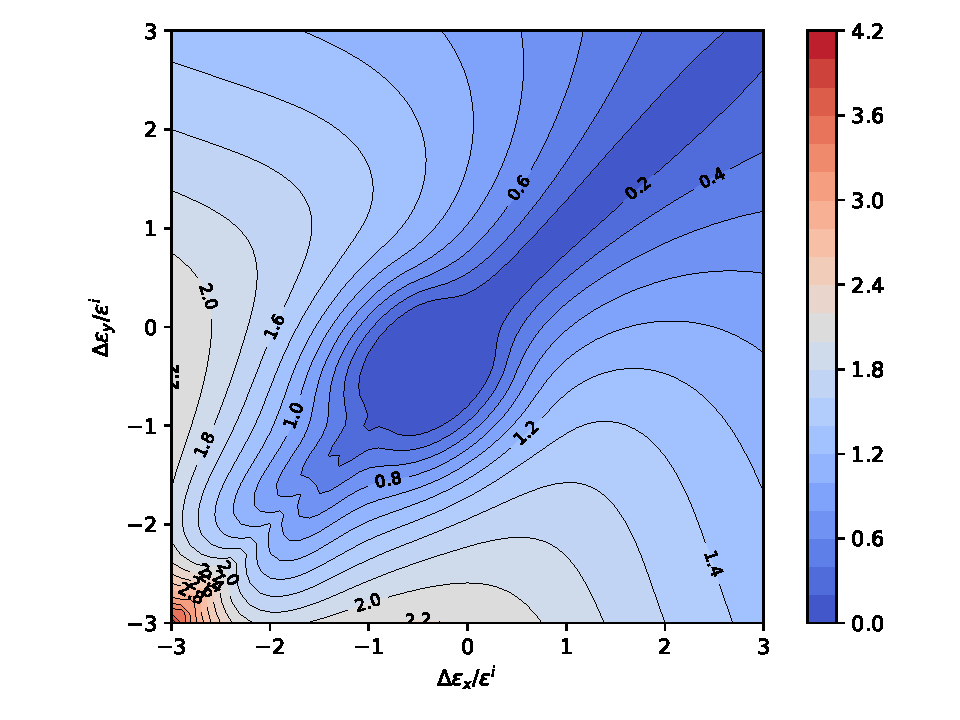
\includegraphics[width=.99\textwidth]{PIC/ISOMAP/error.iso.biaxial.pdf}
    \caption{region A (biaxial)}\label{fig:error_euler_iso_a}
\end{subfigure}\hfill
\begin{subfigure}{.48\textwidth}\centering
    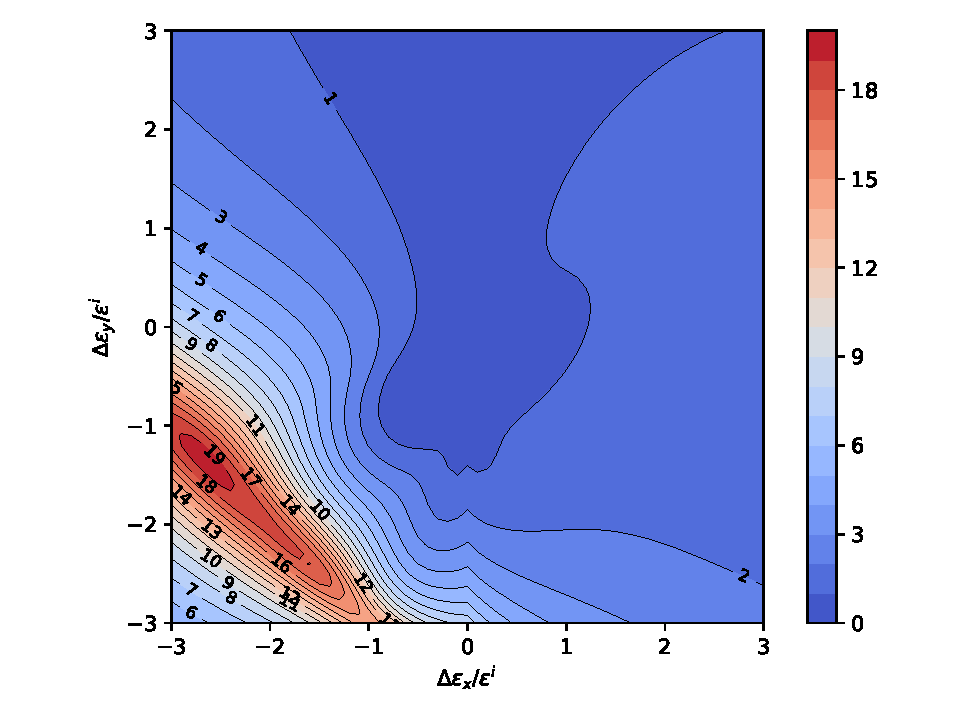
\includegraphics[width=.99\textwidth]{PIC/ISOMAP/error.iso.uniaxial.pdf}
    \caption{region B (uniaxial)}\label{fig:error_euler_iso_b}
\end{subfigure}
\caption{error map (\si{\percent}) using the closest point projection method (isotropic hardening only)}\label{fig:error_euler_isotropic}
\end{figure}
\paragraph{With Elastic Core}
The evolution of elastic core, along with both isotropic and kinematic hardening, is considered in this example.
The following parameters are used in the numerical analysis: $E=\SI{2E5}{\mega\pascal}$, $\nu=0.2$, $\sigma^i=\SI{100}{\mega\pascal}$, $k_\text{iso}=\SI{2E3}{\mega\pascal}$, $u=\num{5E2}$, $a^i=\SI{200}{\mega\pascal}$, $b=\num{5E2}$, $c_e=\num{5E2}$ and $z_e=\num{0.7}$.
The rest of the parameters are set to zero.
The corresponding error map is shown in \figref{fig:error_euler_with_core}.
\begin{figure}[htb]
\centering
\begin{subfigure}{.48\textwidth}\centering
    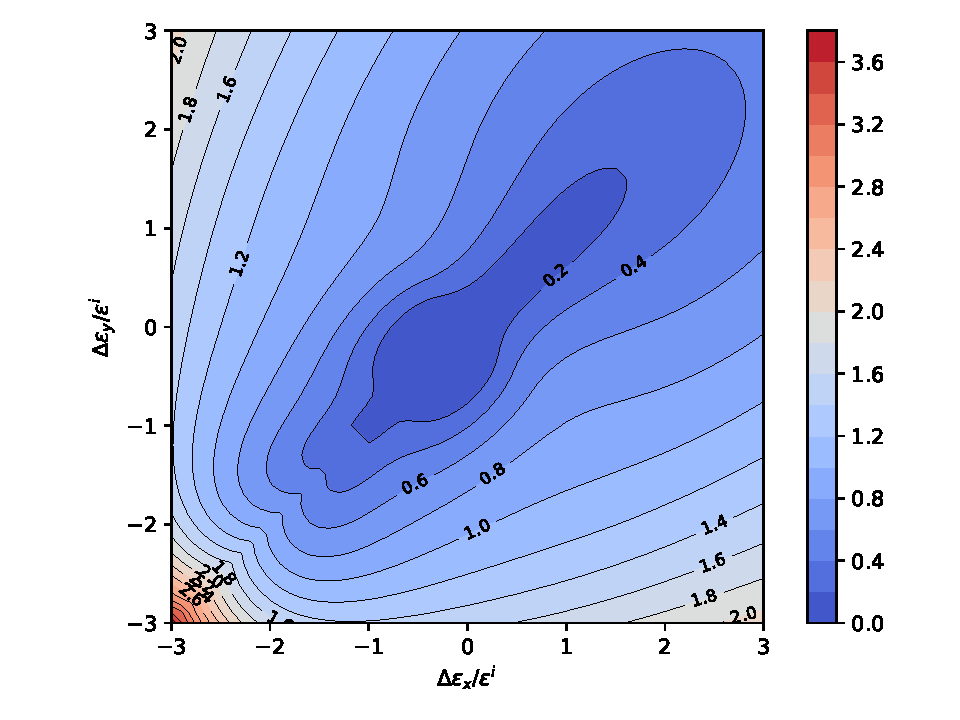
\includegraphics[width=.99\textwidth]{PIC/ISOMAP/error.core.biaxial.pdf}
    \caption{region A (biaxial)}\label{fig:error_euler_with_core_a}
\end{subfigure}\hfill
\begin{subfigure}{.48\textwidth}\centering
    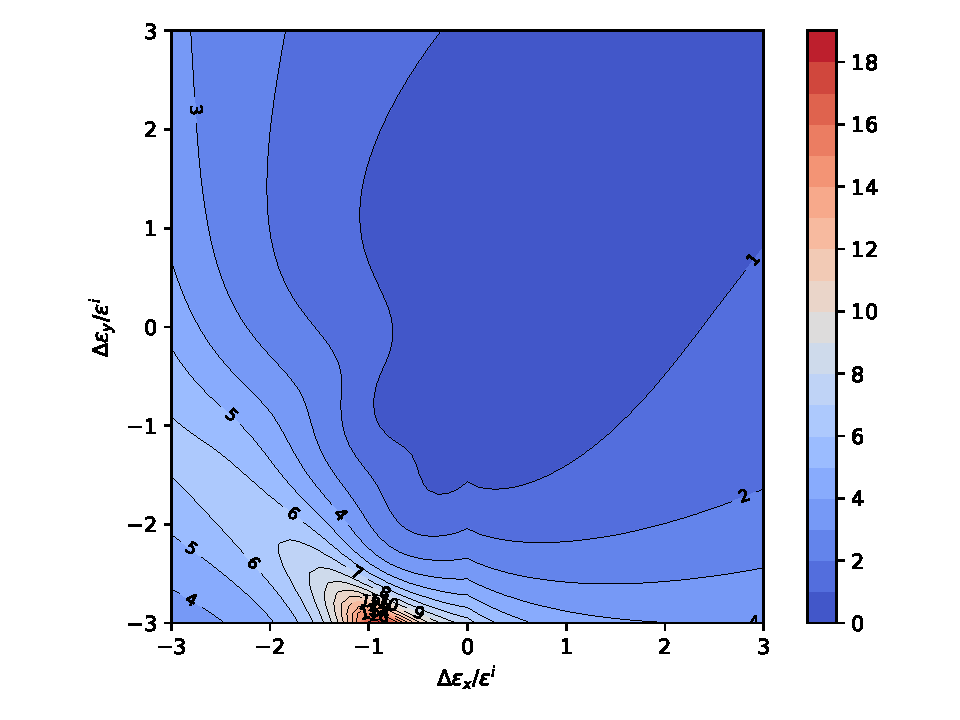
\includegraphics[width=.99\textwidth]{PIC/ISOMAP/error.core.uniaxial.pdf}
    \caption{region B (uniaxial)}\label{fig:error_euler_with_core_b}
\end{subfigure}
\caption{error map (\si{\percent}) using the closest point projection method (with elastic core)}\label{fig:error_euler_with_core}
\end{figure}

For biaxial loading path, it can be observed that the unloading direction (towards the origin) tends to have a higher error than the rest.
For uniaxial loading path, significant errors are observed around the regions where $z$ is close to zero.
The rest of the regions appear to have a relatively good accuracy according to the \SI{5}{\percent} rule \citep[see][pg.~132]{Simo1998}.
% This is mainly caused by the fact that the numerical integration of $z$ is less accurate around $z=0$, especially when the step size is large, as the adopted rate function $U\left(z\right)$ is not bounded and approaches infinity as $z$ approaches zero.
% However, even using a more accurate numerical method, such as the trapezoidal rule, the corresponding numerical performance would not be significantly improved.

In fact, using the indicator adopted by \citet{Anjiki2019}, which is effectively the absolute error, one could see that the large relative error is mainly caused by the small reference stress $\bsigma_\text{ref}$.
\figref{fig:abs_error} further show the absolute error map in region B for the two cases considered.
\begin{figure}[htb]
    \centering
    \begin{subfigure}{.48\textwidth}\centering
        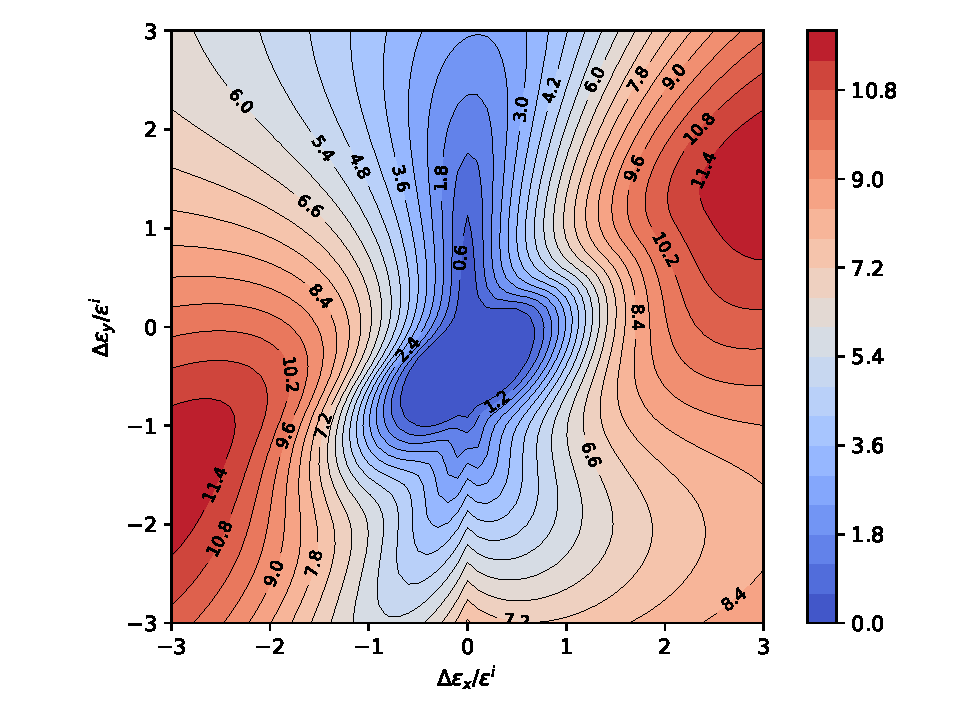
\includegraphics[width=.99\textwidth]{PIC/ISOMAP/abs.error.iso.uniaxial.pdf}
        \caption{with isotropic hardening only}\label{fig:abs_error_euler_with_iso}
    \end{subfigure}\hfill
    \begin{subfigure}{.48\textwidth}\centering
        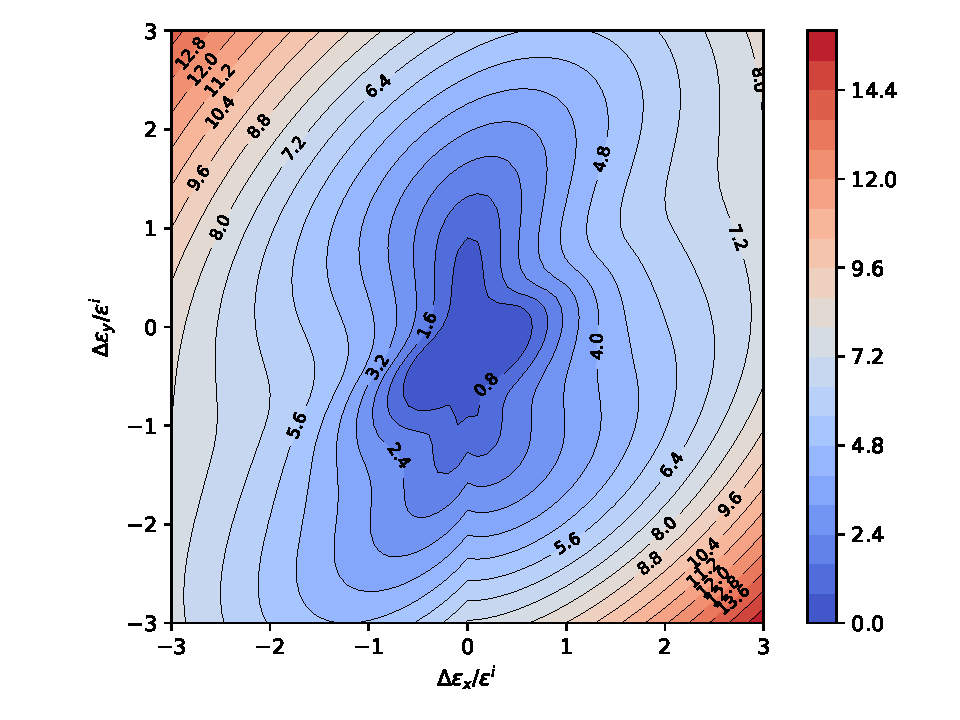
\includegraphics[width=.99\textwidth]{PIC/ISOMAP/abs.error.core.uniaxial.pdf}
        \caption{with elastic core}\label{fig:abs_error_euler_with_core}
    \end{subfigure}
    \caption{absolute error map in region B}\label{fig:abs_error}
\end{figure}
It could be observed that there is no significant difference between outwards and inwards directions, indicating that the proposed unloading criterion possesses a similar accuracy to that of returning mapping towards loading directions.
The overall error is below \SIrange{5}{6}{\percent} of $\sigma^i$ in most regions.
\subsection{Cyclic Response}
The reference comparison can be seen in the work by \citet{Hassan2008,Hashiguchi2017a}.
The following parameters are used:
$E=\SI{2E5}{\mega\pascal}$,
$\sigma^i=\SI{232}{\mega\pascal}$,
$\sigma^s_\text{iso}=\SI{70}{\mega\pascal}$,
$m^s_\text{iso}=\num{30}$,
$a^i=\SI{209}{\mega\pascal}$,
$a^s_\text{kin}=\SI{63}{\mega\pascal}$,
$m^s_\text{kin}=\num{30}$,
$u=\num{2E3}$,
$b=\num{2}$,
$c_e=\num{143}$,
$z_e=\num{0.7}$.
The rest of the parameters are set to zero.

\figref{fig:cyclic_total} depicts the cyclic response.
Due to the presence of the elastic core, the evolution $d$ allows plastic strain to accumulate even when the material undergoes `elastic unloading' (in the conventional sense).
The history of the back stress $\bbeta$ is not shown as it is insignificant with the parameters used.
\begin{figure}[htb]
\centering
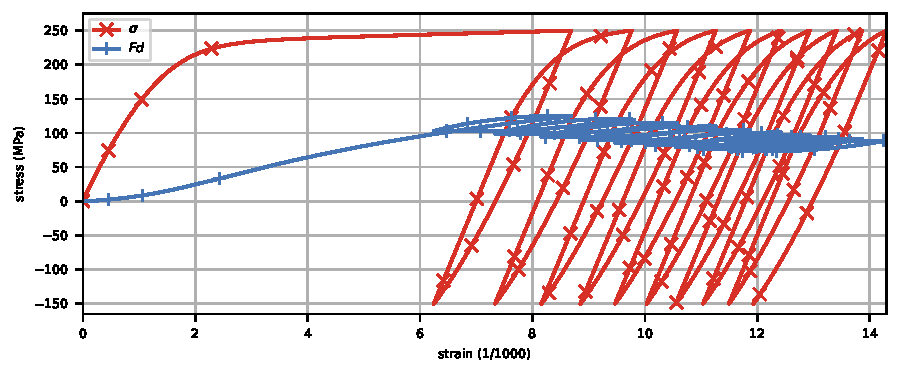
\includegraphics{PIC/CYCLIC/cyclic.total.pdf}
\caption{total stress and evolution of elastic core}\label{fig:cyclic_total}
\end{figure}

\figref{fig:internal_total} and \figref{fig:internal_q} show the evolution of the normal yield ratio $z$ and the similarity vector $d$ against the total strain $\varepsilon$ and the accumulated plastic strain $q$, respectively.
\begin{figure}[htb]
    \centering
    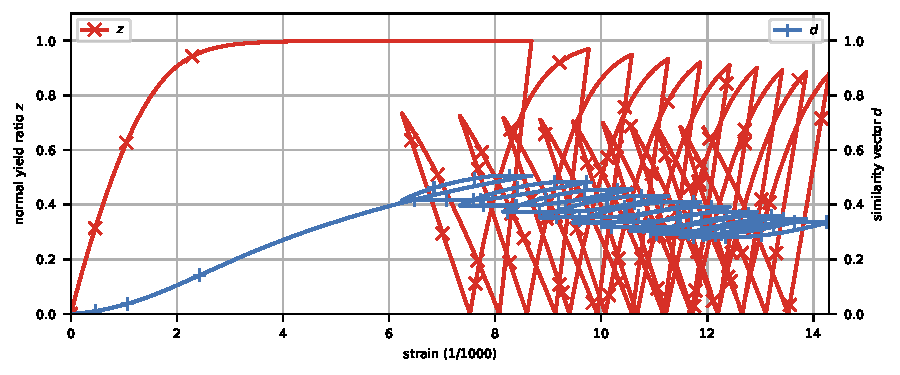
\includegraphics{PIC/CYCLIC/cyclic.ratio.total.pdf}
    \caption{normal yield ratio $z$ and similarity vector $d$ against total strain $\varepsilon$}\label{fig:internal_total}
    \end{figure}
    \begin{figure}[htb]
    \centering
    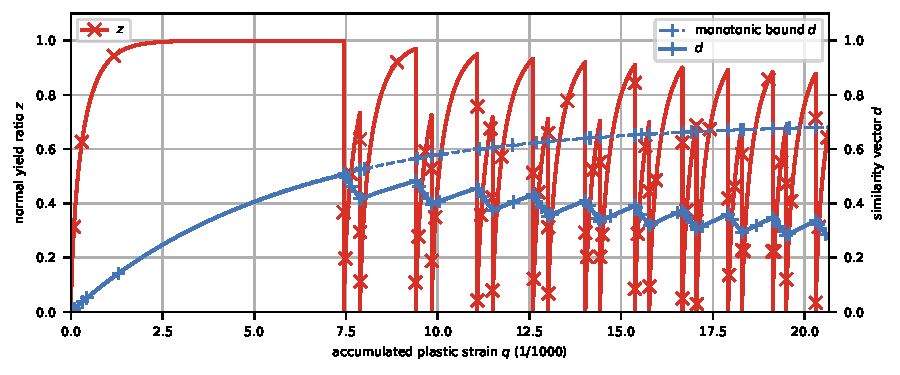
\includegraphics{PIC/CYCLIC/cyclic.ratio.plastic.pdf}
    \caption{normal yield ratio $z$ and similarity vector $d$ against accumulated plastic strain $q$}\label{fig:internal_q}
\end{figure}
Since the model presented in this work is functionally equivalent to the original extended subloading surface model, the overall performance is expected to be similar.
However, as the relevant parameters are defined differently in this work, not all of them are interchangeable with the original model in general.
\section{Conclusions}
In this work, the following contributions are made.
\begin{enumerate}
    \item The evolution rules for back stress and elastic core are revised.
    We ditched the idea of directly defining the back stress $\bbeta$ and the elastic core $\bc$ as independent historic variables.
    Instead, we adopt the `peudo-polar coordinate' decomposition as shown in \eqsref{eq:decomposition_back} and \eqref{eq:decomposition_core}.
    As a result, the proposed rules are equivalent to the original proposal while remain in simple forms that are easy to understand and implement.
    \item A simpler, universal loading/unloading condition with an algebraic interpretation is proposed.
    The procedure does not involve complex criteria and is cheap to evaluate.
    \item The specific form of evolution function $U\left(z\right)$ is further discussed.
          For numerical robustness and stability, functions that do not meet the `strong' numerical continuity condition are recommended.
    \item A reference efficient implementation is presented.
    Compared to previous implementations, the proposed implementation is more compact and efficient.
    The consistent tangent stiffness can also be explicitly evaluated.
\end{enumerate}
To summarise, the proposed formulation offers a functionally equivalent but more concise and compact alternative to the original extended subloading surface model.
This allows for a more straightforward and efficient numerical implementation without compromising accuracy and robustness.

Due to the length limitation, some additional `add-on' features, including cyclic isotropic hardening stagnation and tangential component, are not discussed in this work.
However, extending the proposed model to include these features is straightforward.

Both the uniaxial and 3D version of the proposed subloading surface model suitable for metals have been implemented in \texttt{suanPan} \citep{Chang2024}.
All numerical models and the relevant scripts are available in this repository\footnote{https://github.com/TLCFEM/subloading-implementation}.
\bibliography{BIB}
\end{document}